\chapter{Optimization}

%Introduction
\section{Introduction}
The main goal of the project is to have the car consume the least amount of fuel
possible.  In the ideal world shall the engines and motors therefore always
operate within a certain range of their optimal point of operation. The torque
request from each of the engine/motors should consider this in order to reduce
fuel consumption. In addition to this goal, there is a number of constraints
that needs to be considered in addition to the generic fuel consumption
optimization.  Things like track topography, super-capacitor voltage,
competitors on the track etc.\ will all weight in on the output request. The
optimization algorithm used in Elbas automatic drive mode was developed as a
part of a Master Thesis~\cite{liu2016}. The control architecture for this
optimization consists of two or three layers and the thesis have completed the
top layer speed reference control. This chapter will cover the decentralized
hierarchical predictive control that is used to calculate the speed trajectory
and it's implementation.

\section{Design Decisions}
The need for an optimization can seem to be obvious in order to lower the fuel
consumption. However depending on the tracks topography there might be other
areas that would need much more consideration. In recent years the track of SEM
have been more or less flat, with only minor deviations in altitude. With this
track, there considerations for an automated drive mode would more or less only
consist of making sure that the voltage level of the super capacitor is within
the boundaries. This means that the ICE needs to be started when the voltage
level gets too low and regenerate energy into the super capacitor. The reason for
this is that the efficiency of the electrical motors exceeds that of the ICE,
and in so it will be more efficient to drive Elba with the electrical motors.
Once SEM moved to London the conditions became different, on top of the voltage
level of the super capacitor there is also the room for optimizing the torque
requests so that the most efficient propulsion constellation is active at all
times. It is also nessesary to time the accessible energy so that there is
enough energy in the super capacitor in beginning of an uphill. There is now
also the possibility to regenerate from driving down hill etc.\ These new levels
of complexity makes the optimization become more of an factor then previous
years, and in so there was a collaboration with a master thesis student who used
Elba as an experiment in the thesis~\cite{liu2016}.\\
The Simulink lookup table that was produced from~\cite{liu2016} was dependent on
the current distance traveled on the track so there was a real need to get an
accurate position reading. There was two options, to get an GPS-positioning
device and get that to talk with the rest of the car or to use the encoder
already mounted on the drive shaft. Both had their disadvantages, with the
encoder reading having the tendency to drift and plain inaccuracy and the GPS
with its CEP of $\pm2.5\textnormal{m}$. When the RCP2 was bought it came with an
GPS solution already implemented, this made the choice of having both of them
easier. The next problem that then arouse was to filer the readings of both the
GPS and the encoder to have a reliable positioning source. Due to priorities and
limited amounts of time have the filtering not been completed. 

\section{Constraints}
The optimization is limited by the constraints of the physical system, meaning that
the controller is not able to operate outside the limits of the system. These limits
are,
\begin{align}
    &U_{cap} \in [39,48]~\textup{V} \\
    &\nu \in [0,15]~\textup{m/s}\\
    &a_{\max} \in [-1,1]~\textup{m/s$^2$}
\end{align}
where $U_{cap}$ is the voltage level of the super-capacitor, $\nu$ is the speed
and $a$ is the acceleration in every time step. Due to the fact that there is a
lower limit to the voltage level of the super-capacitor, it is necessary to
change drive mode to engage the ICE in order to regenerate and store energy
until the upper limit is reached. Since the optimization is currently only done
in the top layer, there is a need for the voltage limit to be considered
manually in the model.

\section{Position recognition}\label{sec:opt_pos_recon}
The optimization bases the output reference speed on the current position on the
track. This yields the need for a position recognition with an accuracy precise
enough to be able filter it with sufficient results. The track itself, rather
then time is discretized in order to get a more accurate position in relation to
the tracks topography. \\
There is two ways of finding Elba's position on the track. The first way is a dead
reckoning system based on the shaft encoder~\cite[p.~49]{elba2015},
which calculates the position based on the rotational speed of the shaft. The
second way is based on the GPS system implemented in the race capture pro 2,
where the GPS signal is taken from it's raw form and reshaped with a
Lua-script\footnote{Lua is a dynamically typed scripting language, www.lua.org}
into a CAN-message that is sent on the CAN-bus.


\section{Simulink implementation}
The complete description of the algorithm is found in~\cite{liu2016} and the
implementation is based on this thesis.
\begin{figure}[H]
    \centering
    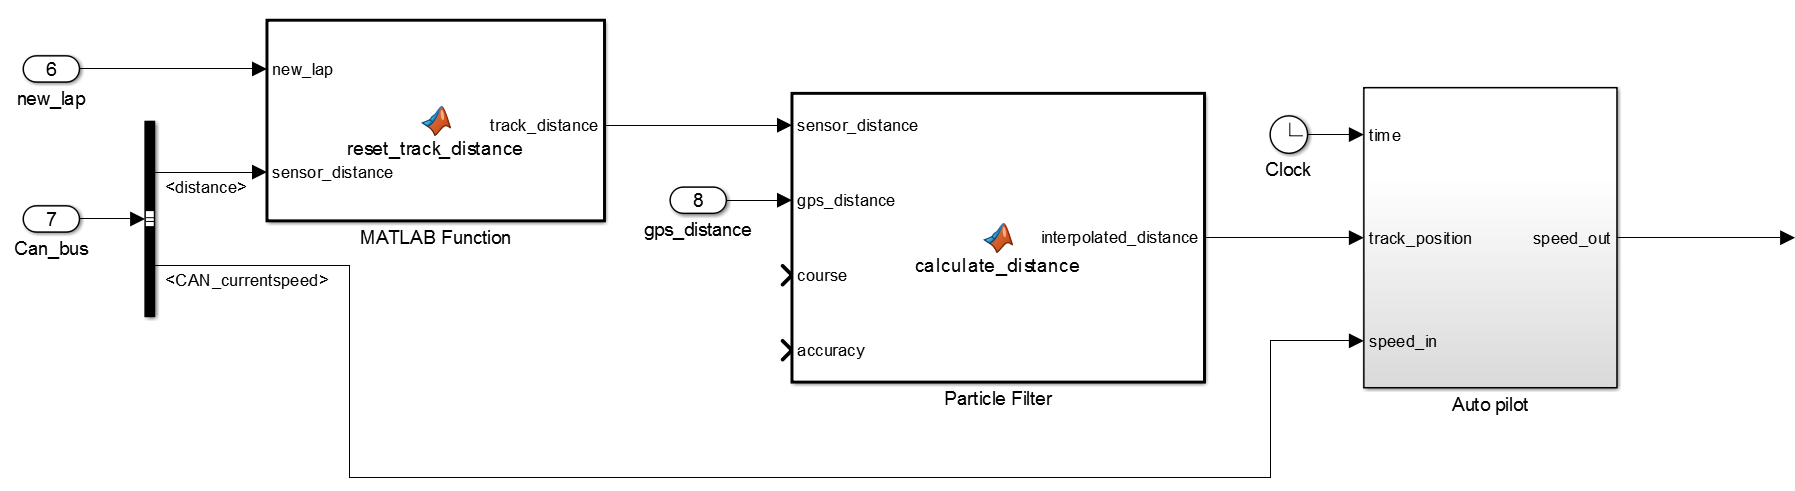
\includegraphics[width=\textwidth]{./img/optimization_cont.png}
    \caption{Simulink implementation for the Hierarchal Optimization
    Algorithm}\label{fig:optimization_cont}
\end{figure}
In Figure~\ref{fig:optimization_cont} the function
\textit{reset\_track\_distance} takes the absolute dead reckoning position
calculated from the shaft encoder and an indicator for a new
lap,~\textit{new\_lap} as input. When the indicator for a new lap is pressed,
the dead reckoning position is zeroed in the function block and the position is
calculated and delivered as the output. The position is sent to a Particle
Filter block where both the dead reckoning and the GPS position is inputed.
These two positioning systems should to be used to get the estimation of the
distance Elba have travelled on the track. The reason for using the particle
filter is because the encoder will likely have a drift and there is an known
inaccuracy in the GPS\@. However, the Particle Filter itself is not implemented at
the moment and is considered to be something future groups need to work on.

There are three inputs into the three dimensional optimization lookup-table, the first one is time. This input is used to synchronize the different time scales in the table and Simulink. The speed input is read from the CAN-bus and is the current speed of
Elba. The track position is the calculated distance travelled on the track from
the filter. The output of the block is an acceleration reference which needs to
be converted to an reference speed since Elba is currently controlled with speed
request. 

\section{Simulation}

\subsection{Static reference speed}
One lap around the track was simulated using the plant model with a constant reference speed of 7 m/s (the slowest allowed speed to be able to complete the race in time). %The resulting speed and vehicle height position can be seen in Figure \ref{fig:optimization_static_speed} 

%TODO: Frågan är om denna ska med alls...
%\begin{figure}[H]
%    \centering\label{fig:optimization_static_speed}
%    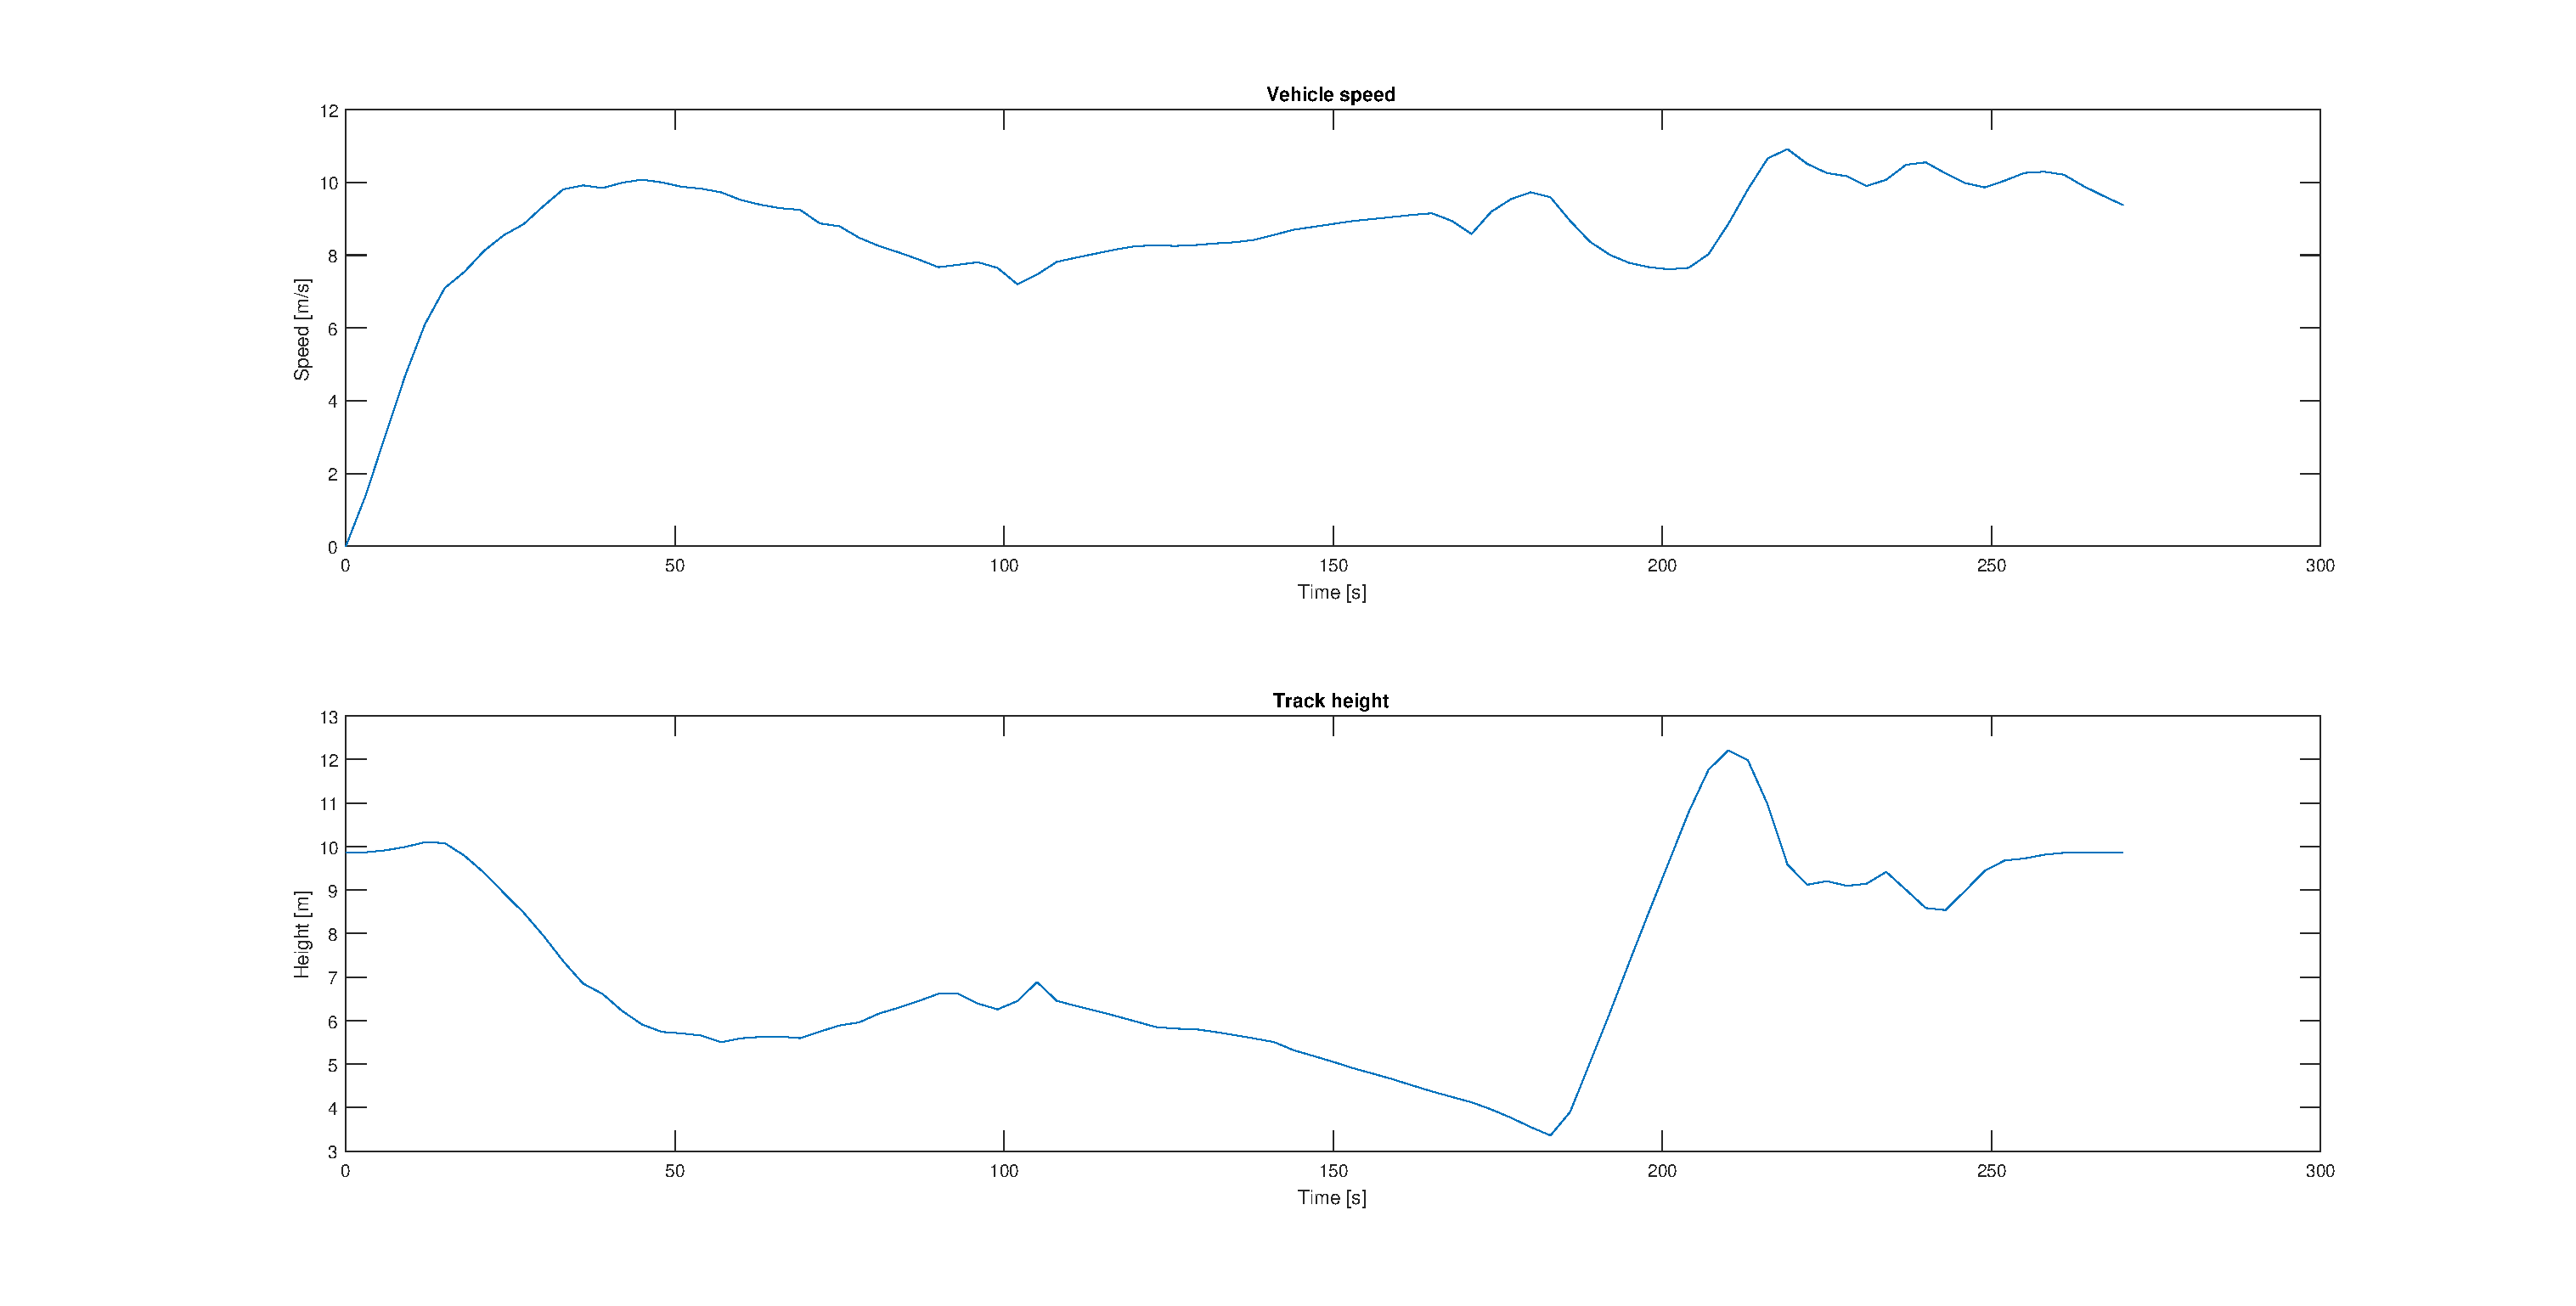
\includegraphics[width=\textwidth]{./img/optimization_static_speed.eps}
%    \caption{Plots of vehicle height and speed as a function of time.}
%\end{figure}

The fuel consumption in $\textnormal{km/l}$ fuel, $f_c$ was calculated according to

\begin{equation} \label{eq:optimization_fuelconsumption}
	f_{tot} = \frac{d_l}{f_i+f_c},
\end{equation}

where $d_l$ is the distance of one lap, $f_i$ the fuel consumed by the ICE and
$f_c$ the equivalent amount of fuel that the super capacitor has been discharged
by since the start of the race, calculated as

\begin{equation} \label{eq:optimization_ethanolenergy}
	f_c = \frac{({{u_{c_0}}^2-{u_{c_{end}}}^2})c_c}{2k},
\end{equation}

where $u_{c_0}$ is the initial capacitor voltage, $u_{c_{end}}$ is the capacitor
voltage at the end of the race, $c_c$ is the capacitance in the capacitor and
$k$ is the conversion ratio from litre ethanol to energy in joule, retrieved
from~\cite{fuelconversion}.

This resulted in $f_{tot} = 172.8$ $km/l$. %TODO: göra snyggare

\subsection{Optimized reference speed}
Using the optimized speed controller as a lookup table (produced by
\citep{liu2016}) dependant on vehicle speed, distance and elapsed time, a new
simulation could be produced. The resulting speed and vehicle height position
can be seen in Figure~\ref{fig:optimization_optimal_speed}

\begin{figure}[H]
    \centering
    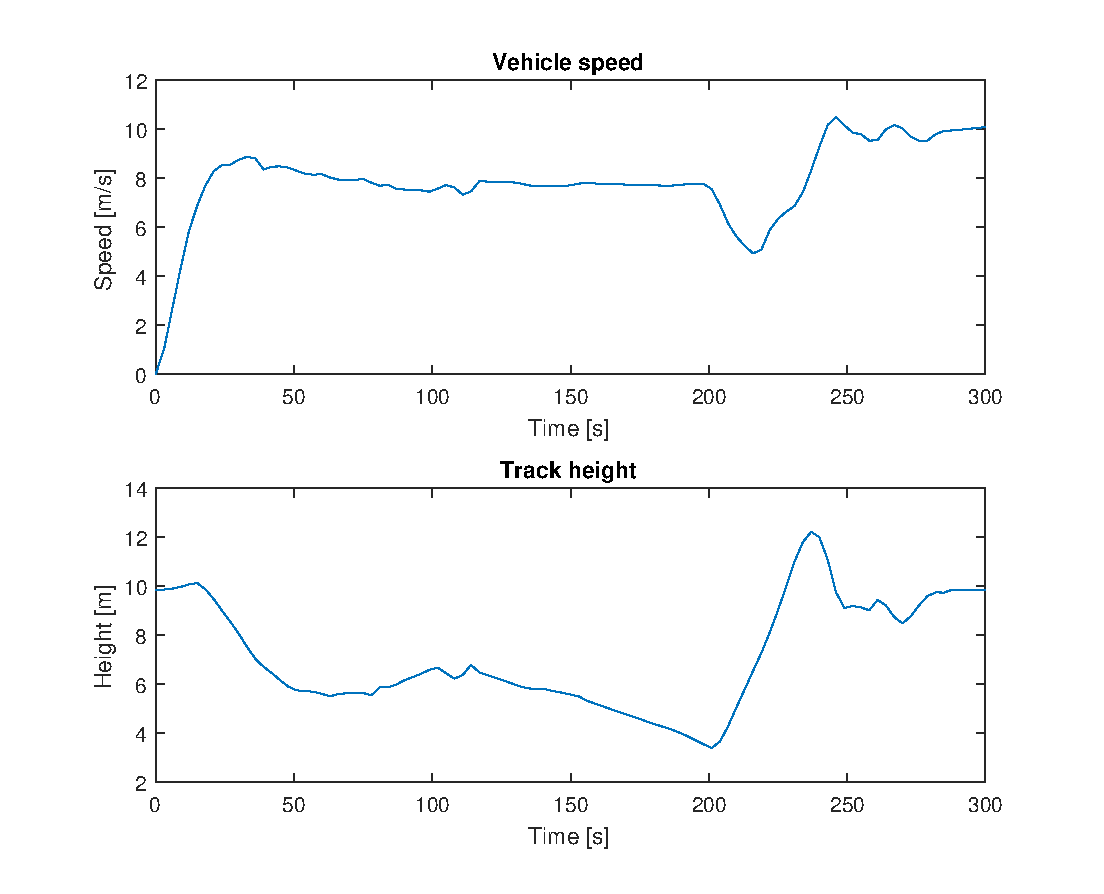
\includegraphics[width=\textwidth]{./img/optimization_optimal_speed.eps}
    \caption{Plots of vehicle height and speed as a function of
    time.}\label{fig:optimization_optimal_speed}
\end{figure}

The amount of kilometers travelled per liter fuel $f_{tot}$ was calculated
according to equation~\ref{eq:optimization_fuelconsumption}. This resulted in
$f_{tot} = 194.1$ $km/l$. %TODO: göra snyggare
